\documentclass{article}

%package setup
\usepackage{graphicx}
\graphicspath{ {./images/} }
\usepackage{amsmath}
\usepackage{fancyhdr}
\usepackage[margin=1in]{geometry}
\usepackage{subcaption}
\usepackage{comment}
\usepackage[hidelinks]{hyperref}
\usepackage{enumitem}
\usepackage{float}
\usepackage{textcomp, gensymb}
\usepackage{caption}
\setlength\parindent{0pt}


% \pagestyle{fancy}
% \fancyhf{} % Clear header/footer settings
% \rhead{\thepage} % Page number on the right in the header
% \lhead{ASE 375 Final Project Proposal} % Your lab report title on the left

% \title{Propeller Twist Efficiency}
% \author{Group 6: Andrew Doty, Andres Suniaga, Dennis Hom}

\begin{document}
\begin{flushleft}
    \small{ASE 375 Group 6 (14115): Andrew Doty, Andres Suniaga, Dennis Hom}\\[2mm]    
    \Large{\textbf{Project Proposal: Propeller Twist Efficiency}}\\[2mm]
\end{flushleft}
% \maketitle
% \begin{titlepage}
  % \centering
  % 
\includegraphics[height=2.5cm]{ase-logo-formal.png}  % Adjust the height as needed
  % \vspace{1cm}  % Add some vertical space
 
%   \Large \textbf{ASE 375 Electromechanical Systems}\\
%   \large \textbf{Section 14115}\\
%   \vspace{0.5cm}
%   \textbf{Monday: 3:00 - 6:00 pm}\\
 
%   \vspace{1cm}
 
%   \hrule
%   \vspace{0.5cm}
 
%   \Huge \textbf{Final Project Proposal: \\
%                 Propeller Twist Efficiency}
%  \Huge \textbf{}\\
 
%   \vspace{0.5cm}
%   \hrule
 
%   \vspace{1cm}
 
%   \normalsize \textbf{Group 6: Andrew Doty, Andres Suniaga, Dennis Hom}\\
%   \normalsize \textbf{Due Date: 04/01/2024}
 
% \end{titlepage}

\section{Question}
Imagine we are designing an RC aircraft. \textbf{How does propeller twist affect efficiency?} Twist defines the angle of incidence of the propeller. This varies from the hub to the tip of the prop due to the different speeds along the blade as it spins.
\section{Experiment}
How will we determine the propeller's efficiency? Using an arm designed to mount a DC Motor and Speed Controller, we will measure the thrust force and the power used. The speed of the motor will be controlled via PWM generator communicating through the speed controller. For consistency, the same PWM signal will be supplied for all tests. We will use strain gages placed at the root of the arm as shown in Figure \ref{fig:finalsetup} to measure the propeller thrust at the tip. With a power supply, we can ensure that the same input voltage is supplied and from a watt-meter we can gather the electrical power consumption.
\begin{figure}[H]
    \centering
    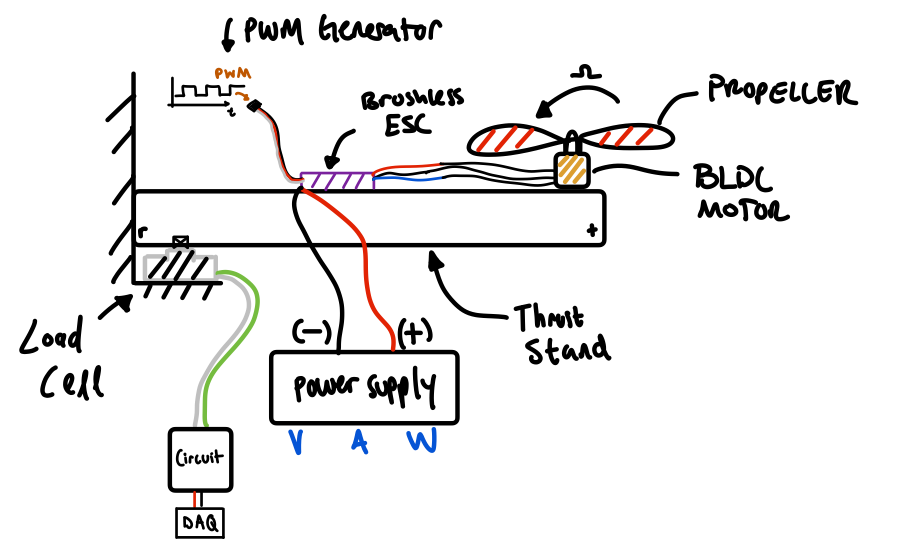
\includegraphics[width = 0.5\textwidth]{EMech_FinalExperiment_IdeaSetup_Updated.png}
    \caption{Hypothetical Experiment Setup}
    \label{fig:finalsetup}
\end{figure}
We will experiment with a number of propellers of different twist but same diameter. We can test the consistency of the motor's RPM and how it compares to the manufacturer's $\text{K}_{\text{v}}$ with a hall-effect sensor. With a ratio of the propeller thrust and electrical power consumption we can determine the "efficiency" (power loading) of the propeller and how it is affected by twist. 
\section{List of Equipment}
\begin{enumerate}
    \item Strain Gages, with dummy resistors and DAQ
    \item Hall Effect Sensor and Miniature Magnet
    \item BLDC Motor with the proper rated Brushless Electronic Speed Controller 
    \item Power Supply supplying operational voltage, with Voltmeter, Ammeter, and Watt-meter
    \item PWM Wave Generator or PWM/Servo Tester
    \item 3-5 Two-Blade Propellers of same diameter, dependent on the motor specifications, and different twist 
    \item Thrust Stand/Arm with mounting for BLDC Motor
\end{enumerate}
\end{document}
